

\documentclass{beamer}
 
\usepackage[utf8]{inputenc}
\usepackage{pgfpages}
\usepackage{array}

\setbeameroption{hide notes}
 
%Information to be included in the title page:
\title[Evolved Parameterized Selection for Evolutionary Algorithms]
{Evolved Parameterized Selection for Evolutionary Algorithms}
 
\author[Richter, Samuel] % (optional, for multiple authors)
{Samuel Richter (snr359@mst.edu)}
 
\institute % (optional)
{
  Natural Computation Laboratory\\
  Department of Computer Science\\
  Missouri University of Science and Technology\\
  Rolla, Missouri 65409
}
 
\date{December 13, 2018}
 
\usetheme{Copenhagen}
 
\begin{document}
 
	\frame{\titlepage}
	
	\begin{frame}
	\small
	\centering
		Approved by\\
		\vspace{0.3in}
		Daniel Tauritz, Advisor\\
		Patrick Taylor\\
		Samuel Mulder\\
		\vspace{0.3in}
		Copyright 2018\\
		SAMUEL NATHAN RICHTER\\
		All Rights Reserved\\
	\end{frame}

% ----------------------------------------INTRODUCTION		
	
	\begin{frame}
		\frametitle{Introduction}
		
		\begin{itemize}
			\item<1-|alert@1> Evolutionary Algorithms (EAs) are applied to a wide variety of problems, such as optimization, modeling, and system design
			\item<2-|alert@2> Unlike human-designed solutions, they make \textit{a priori} no assumptions about where an optimal solution lies
			\item<3-|alert@3> EAs are highly parallelizable, and well-equipped to navigate complex fitness landscapes
			\item<4-|alert@4> However, many EAs are highly sensitive to configurations/parameters 			 
		\end{itemize}
	\end{frame}
	
	\begin{frame}
		\frametitle{Introduction}
		There are several solutions to configuration sensitivity:
		\begin{itemize}
			\item<2-|alert@2> Self-adaptive parameters
			\item<3-|alert@3> Parameter-less EAs
			\item<4-|alert@4> Parameter-tuning/Hyper-heuristics
		\end{itemize}
	\end{frame}	
	
	\begin{frame}
		\frametitle{Introduction}
		\begin{itemize}
			\item<1-|alert@1> With Hyper-heuristics, we generate new algorithms, or parts of algorithms, tuned for a specific purpose, such as improvement of EAs
			\item<2-|alert@2> We can target components of an EA for improvement on a particular problem class
			\item<3-|alert@3> Previous work has shown that many EA components are good candidates for targeted improvement: mutation/mating preference/genetic representation/crossover operators
			\item<4-|alert@4> Our work targets \underline{selection} for improvement
		\end{itemize}
	\end{frame}	
	
	\begin{frame}
		\frametitle{Introduction}
		\begin{itemize}
			\item<1-|alert@1> Selection processes show up in many EAs, and other meta-heuristic strategies
			\item<2-|alert@2> Selection is used for:
			\begin{itemize}
				\item<3-|alert@3> Selecting individuals to be used for recombination
				\item<4-|alert@4> Selecting individuals to survive to the next generation
				\item<5-|alert@5> Selecting individuals to update internal variables (mean search space, evolution path, etc.)
			\end{itemize}			
			\item<6-|alert@6> EAs and EC often use selection to control the path of evolution
			\item<7-|alert@7> Performance depends heavily on good selection methods
		\end{itemize}
	\end{frame}	
	
	\begin{frame}
		\frametitle{Introduction}
		\begin{itemize}
			\item<1-|alert@1> A number of conventional selection functions exist (tournament, truncation, fitness proportional) and are easy to implement
			\item<2-|alert@2> Some selection functions are parameterized, adding more parameters to be set or tuned
			\item<3-|alert@3> Using the right selection functions and selection parameters (where applicable) has a large impact on EA performance
		\end{itemize}
	\end{frame}		
	
	\begin{frame}
		\frametitle{Introduction}
		\begin{itemize}
			\item<1-|alert@1> Even state-of-the-art EAs have insufficient performance on very difficult problems
			\item<2-|alert@2> The ``No Free Lunch Theorem'' implies that any possible selection function is optimal for some particular EA applied to some particular problem
			\item<3-|alert@3> It is highly unlikely, for a given EA and problem, that the optimal selection exists within the conventional functions
			\item<4-|alert@4> Therefore, we can expect a performance increase by developing a new selection function, tuned to the EA and problem
		\end{itemize}
	\end{frame}	
	
	\begin{frame}
		\frametitle{Introduction}
		\begin{itemize}
			\item<1-|alert@1> Our approach is to use a Hyper-heuristic, with both generative and perturbative components, to develop new selection functions, tuned to particular EAs and problem classes
			\item<2-|alert@2> We develop a meta-EA and a new selection function representation to explore the space of possible selection functions
			\item<3-|alert@3> We determine quality of evolved selection functions by running the EA with them, keeping all other parameters (if any) constant
			\item<4-|alert@4> The EA's performance when using the evolved selection function (as opposed to a conventional selection function) is used as an indicator of the selection function's quality		
		\end{itemize}
	\end{frame}					
	
% ---------------------------OVERVIEW	
	
	
	\begin{frame}
		\frametitle{Overview}
		\begin{itemize}
			 \item<1-> Objective: use a Hyper-Heuristic to generate a selection function for a particular EA operating on a particular problem class
			 \item<2-|alert@2> Step 1: define a representation for selection functions to form a search space
			 \item<3-|alert@3> Step 2: discover which selection processes of the EA can be improved
			 \item<4-|alert@4> Step 3: explore the space of selection functions with a meta-EA
			 \item<5-|alert@5> Step 4: test the EA on new instances from the same problem class to test generalization of the performance increase
		\end{itemize}	
	\end{frame}	
	
% ---------------------------REPRESENTATION	
	
	\begin{frame}
		\frametitle{Representation}
		\begin{itemize}
			 \item<1-|alert@1> A straightforward way to represent selection functions would be to employ a Turing-complete Genetic Programming (GP) space of algorithms that takes a population as input, and returns an individual or pool of individuals
			 \item<2-|alert@2> However, searching through the space of Turing-complete algorithms presents several difficulties
			 \begin{itemize}
			 	\item<3-|alert@3> Searching through an infinite space of functions
			 	\item<4-|alert@4> Ensuring that all outputs are valid valid selection functions
			\end{itemize}			 		 
		
		\end{itemize}	
	\end{frame}			
	
	
	\begin{frame}
		\frametitle{Representation}
		
		\begin{itemize}
			 \item<1-|alert@1> We instead represent selection functions with a new representation, consisting of two major components
			 \item<2-|alert@2> The first component is a mathematical function, encoded in a Koza-style GP-Tree, that calculates a real-valued number corresponding to the individual's desirability
			 \item<3-|alert@3> The second component is a method of selecting individuals, based on their calculated desirability
		
		\end{itemize}
	\end{frame}
	
	\begin{frame}
		\frametitle{Representation}
		A selection function is represented by a mathematical desirability function (encoded in a parse tree), and the final selection method.
		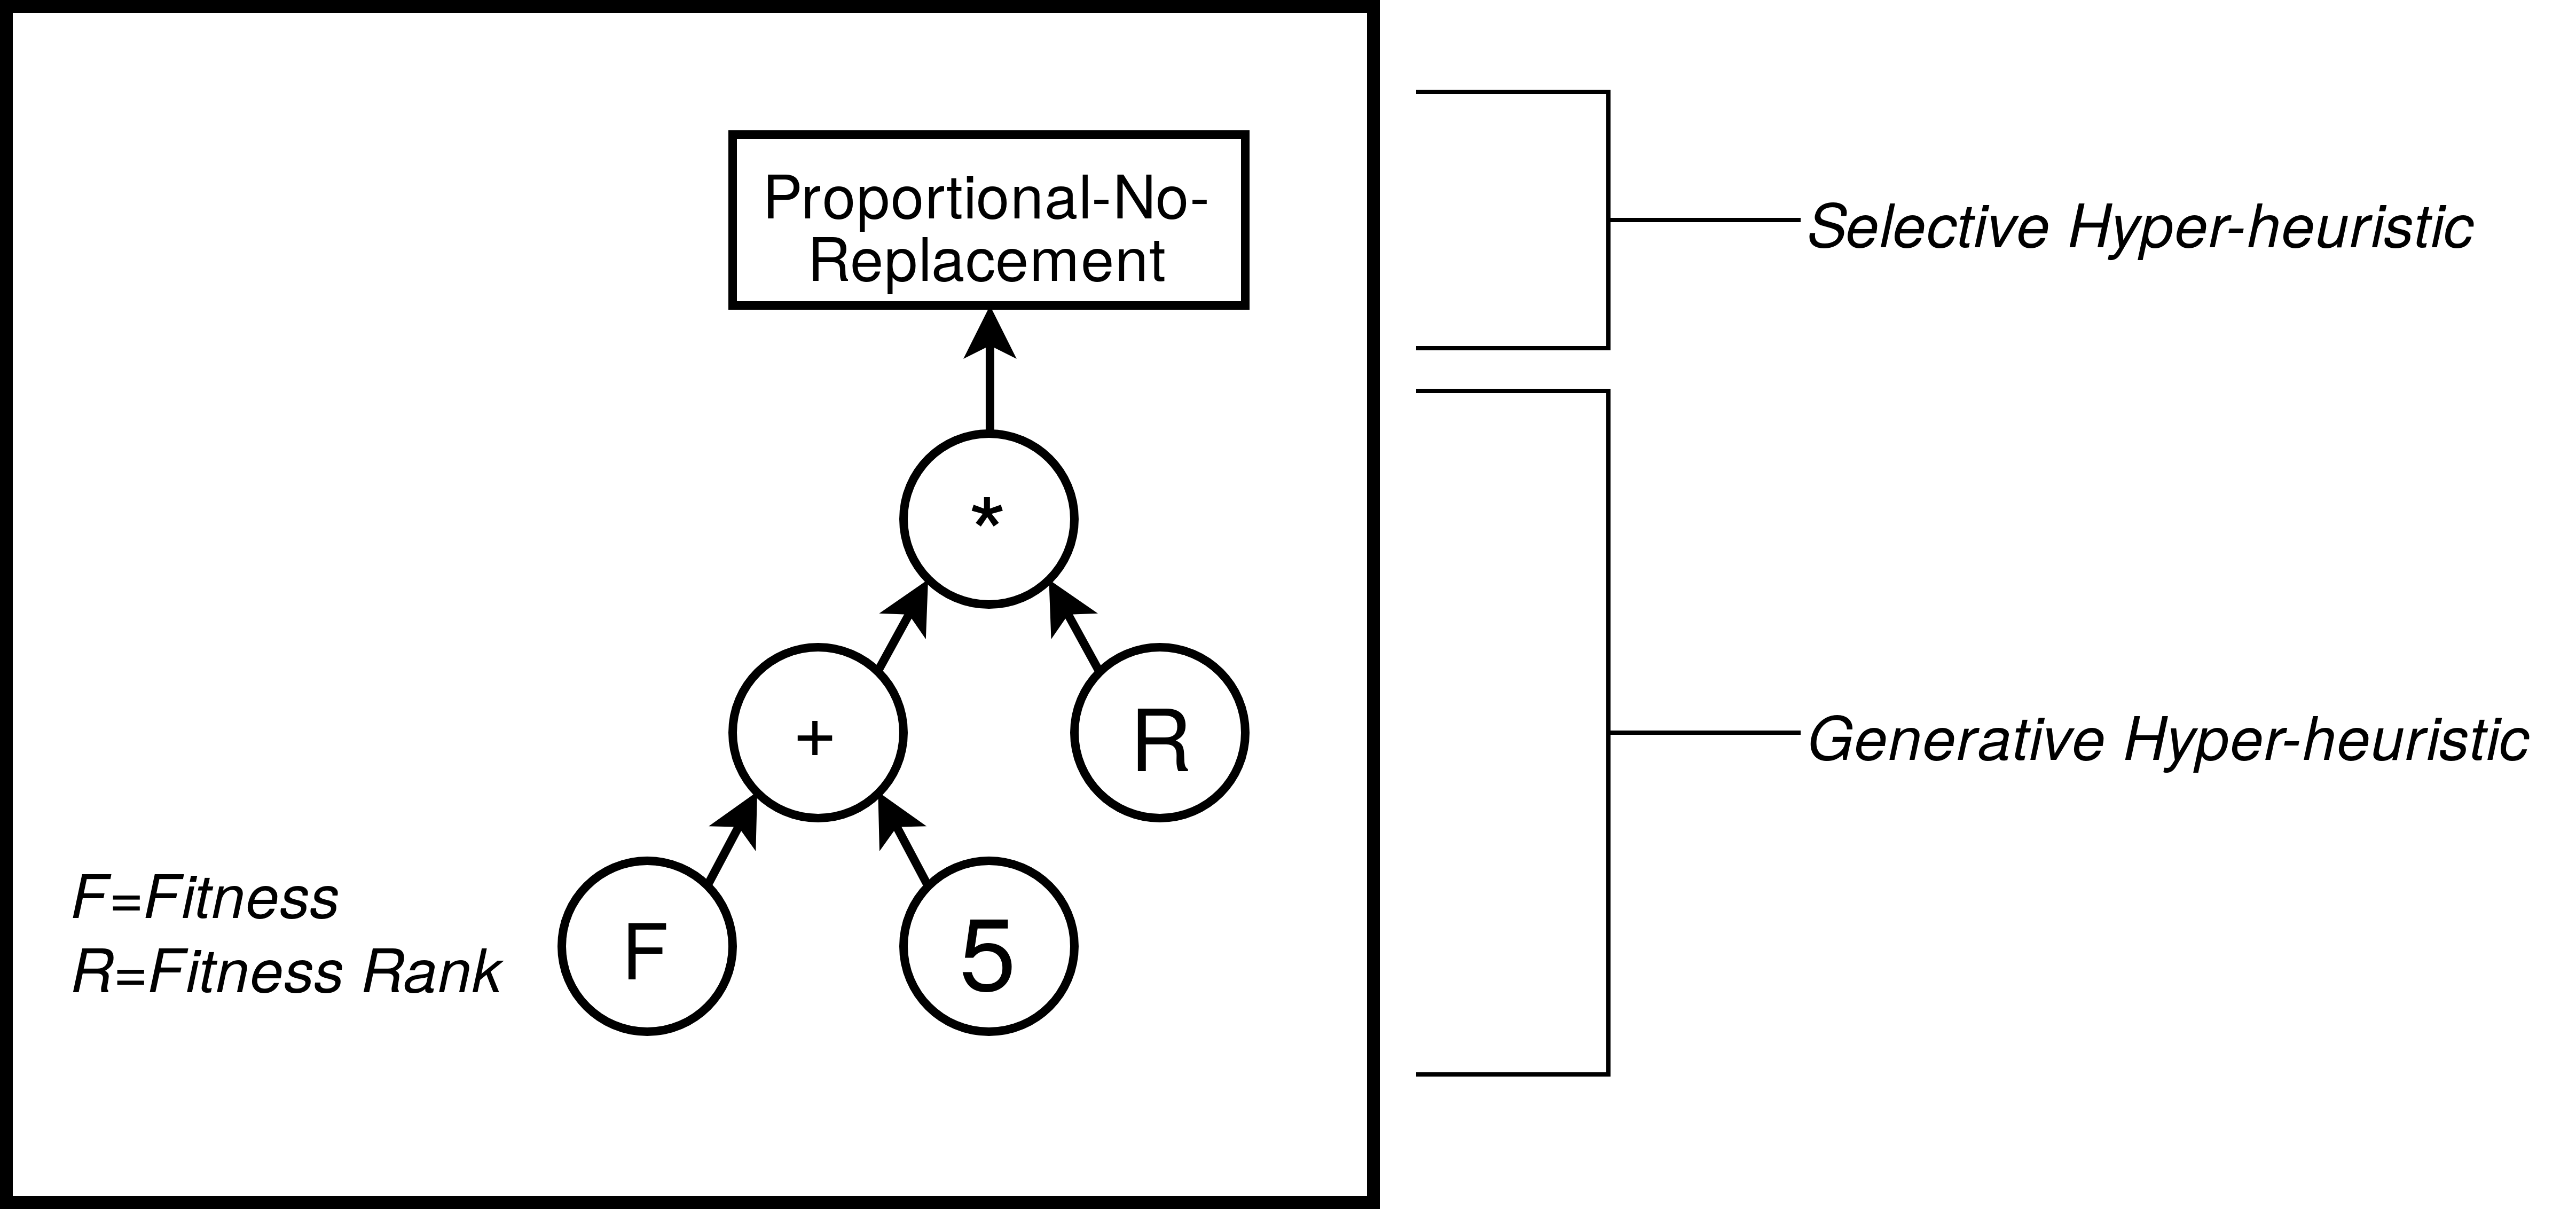
\includegraphics[width=\textwidth]{example_eppsea}
	\end{frame}
	
	\begin{frame}
		\frametitle{Representation - Psuedocode}
		\centering
		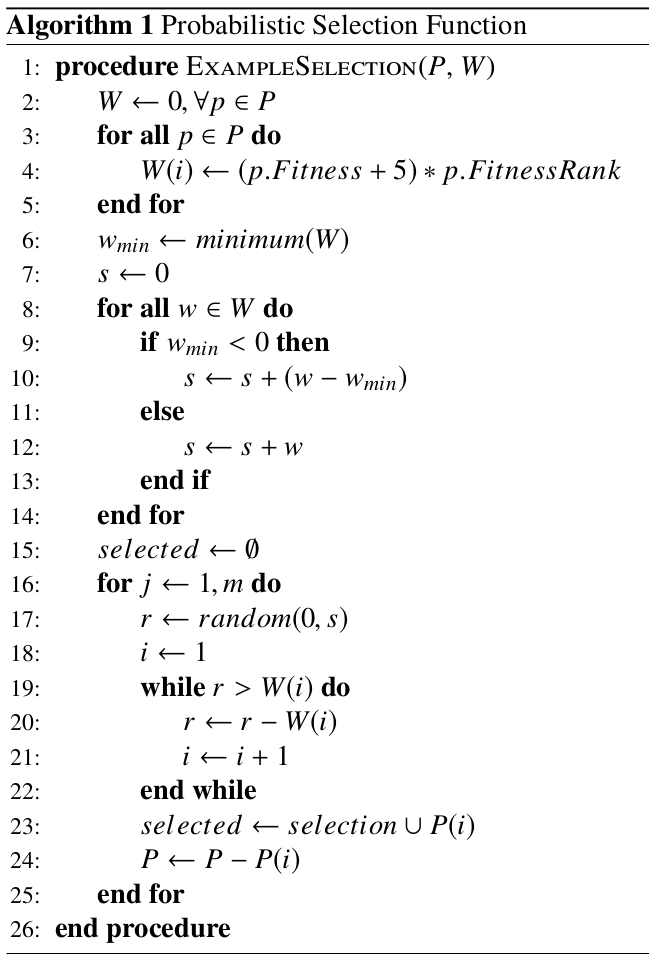
\includegraphics[height=0.8\paperheight]{example_eppsea_code}
	\end{frame}
	
	\begin{frame}
		\frametitle{Representation - Psuedocode}
		\begin{columns}
		\begin{column}{0.5\textwidth}
			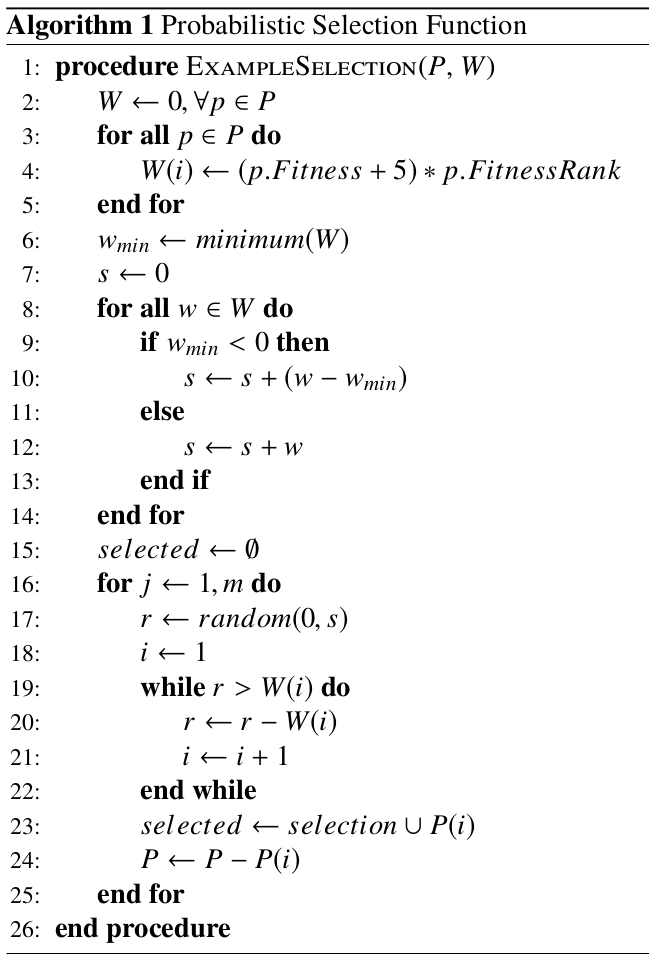
\includegraphics[height=0.8\paperheight]{example_eppsea_code}		
		\end{column}
		\begin{column}{0.5\textwidth}
			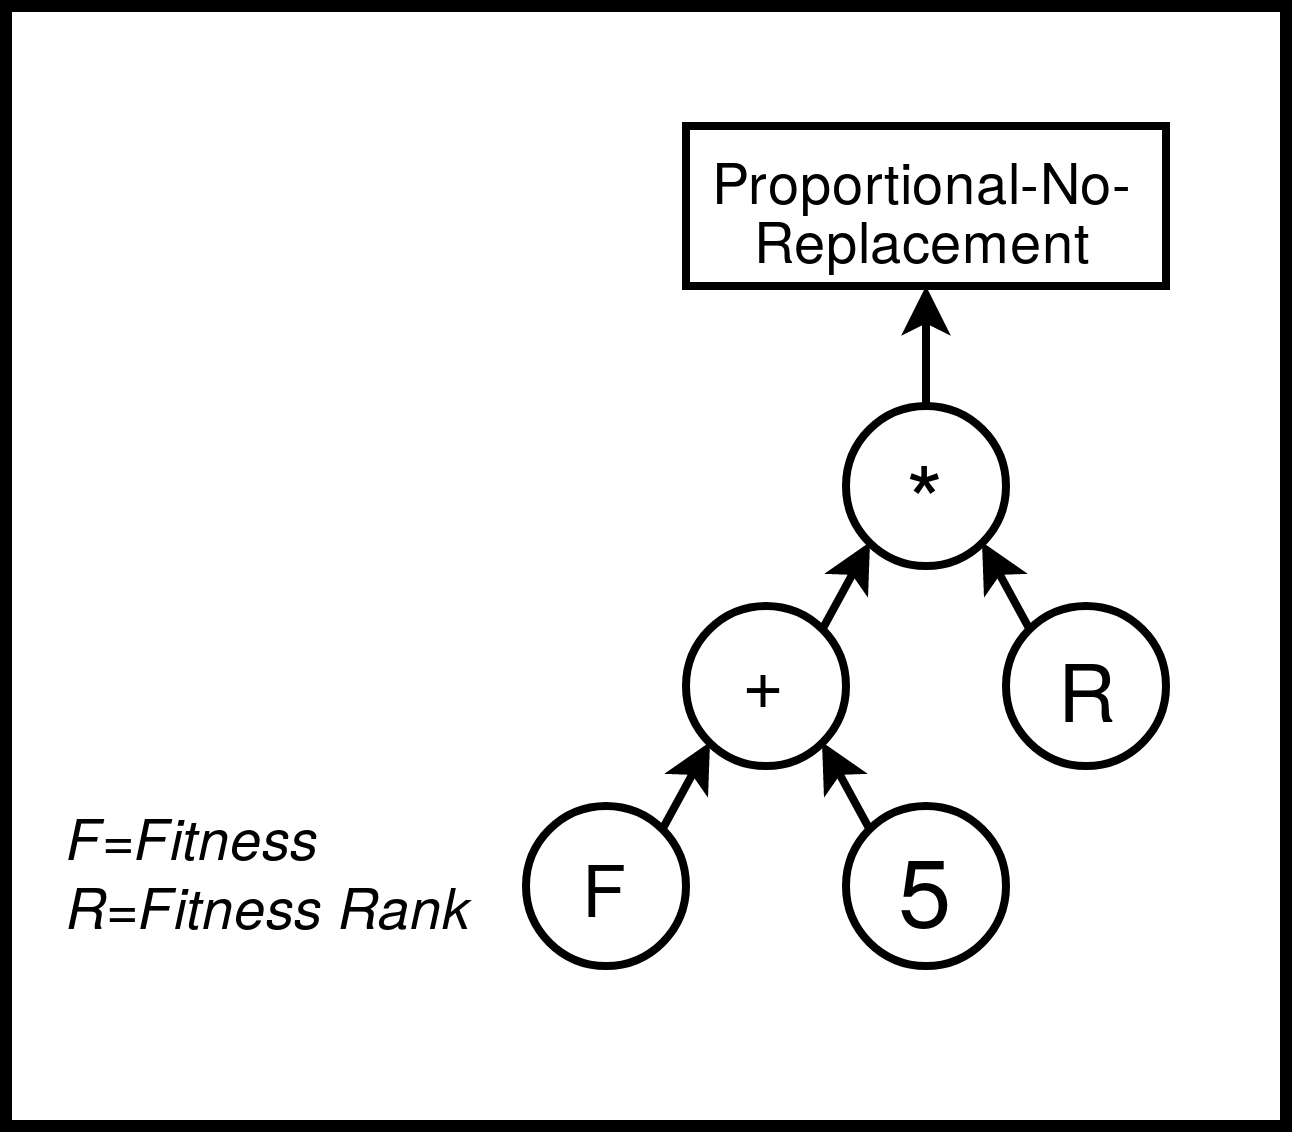
\includegraphics[width=\textwidth]{example_eppsea_no_forks}		
		\end{column}
		\end{columns}		

	\end{frame}	
	
	\begin{frame}
		\frametitle{Representation - Psuedocode}
		\begin{columns}
		\begin{column}{0.5\textwidth}
			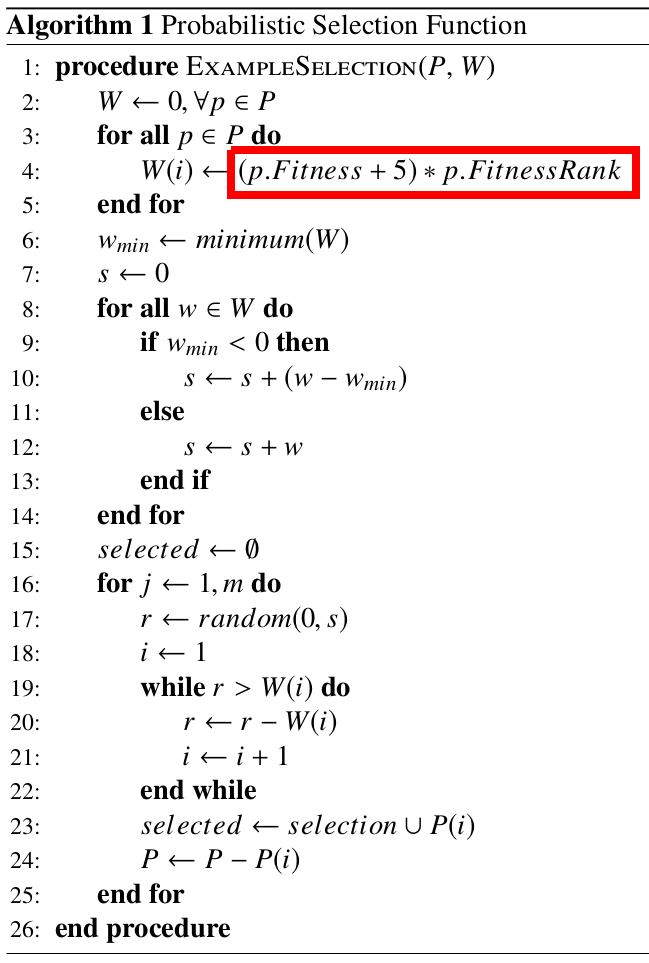
\includegraphics[height=0.8\paperheight]{example_eppsea_code_red_highlight}		
		\end{column}
		\begin{column}{0.5\textwidth}
			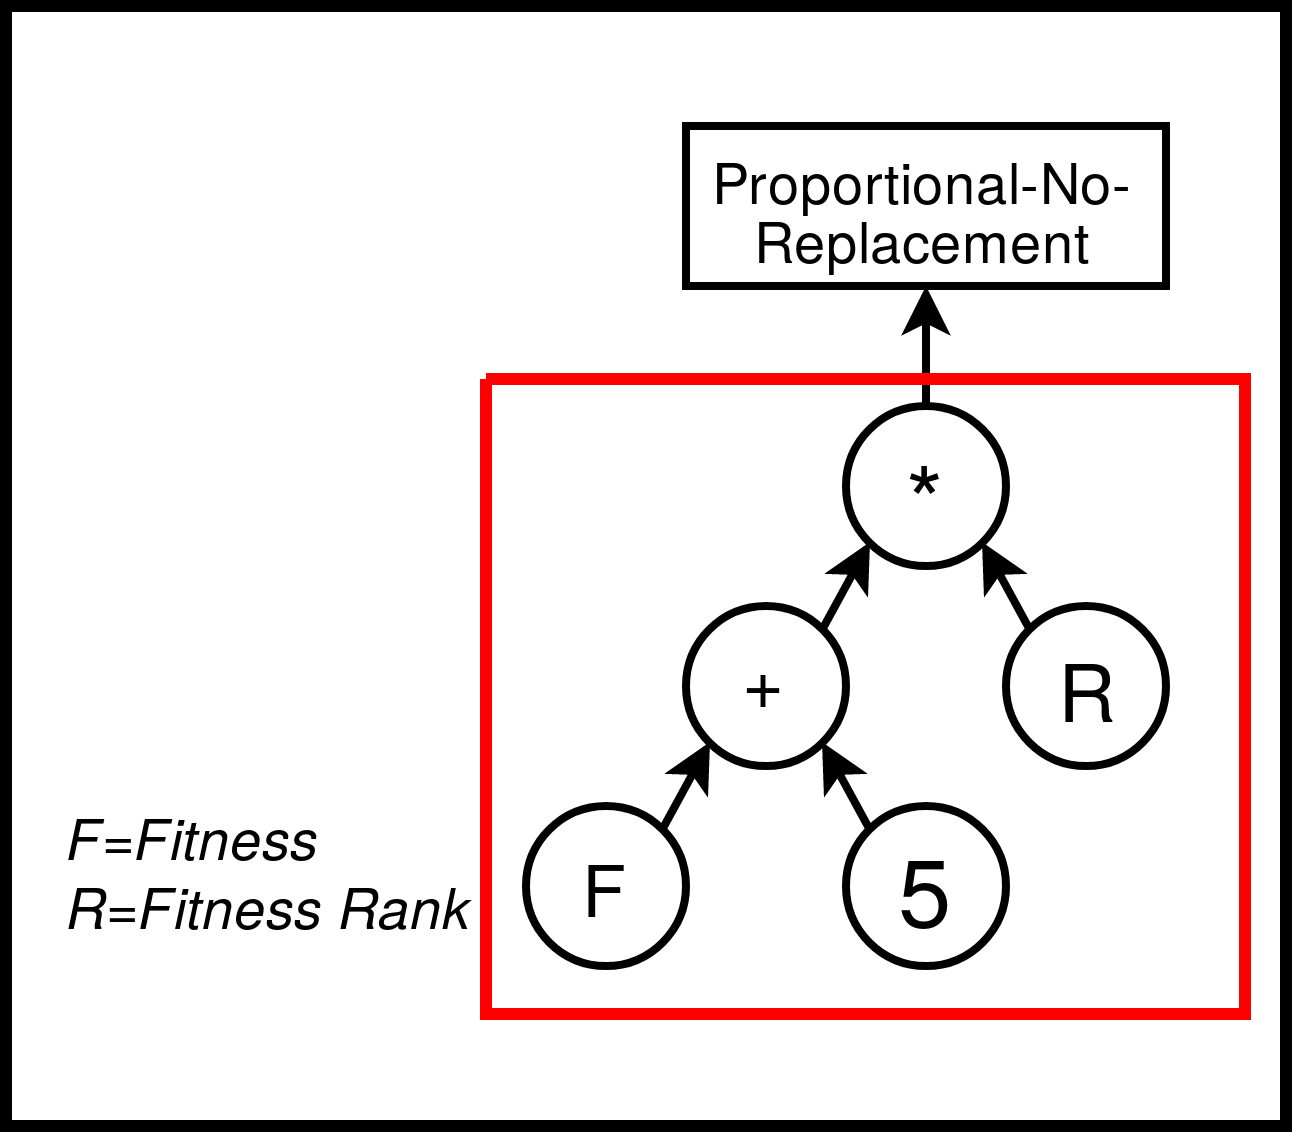
\includegraphics[width=\textwidth]{example_eppsea_no_forks_red_highlight}		
		\end{column}
		\end{columns}		

	\end{frame}	
	
	\begin{frame}
		\frametitle{Representation - Psuedocode}
		\begin{columns}
		\begin{column}{0.5\textwidth}
			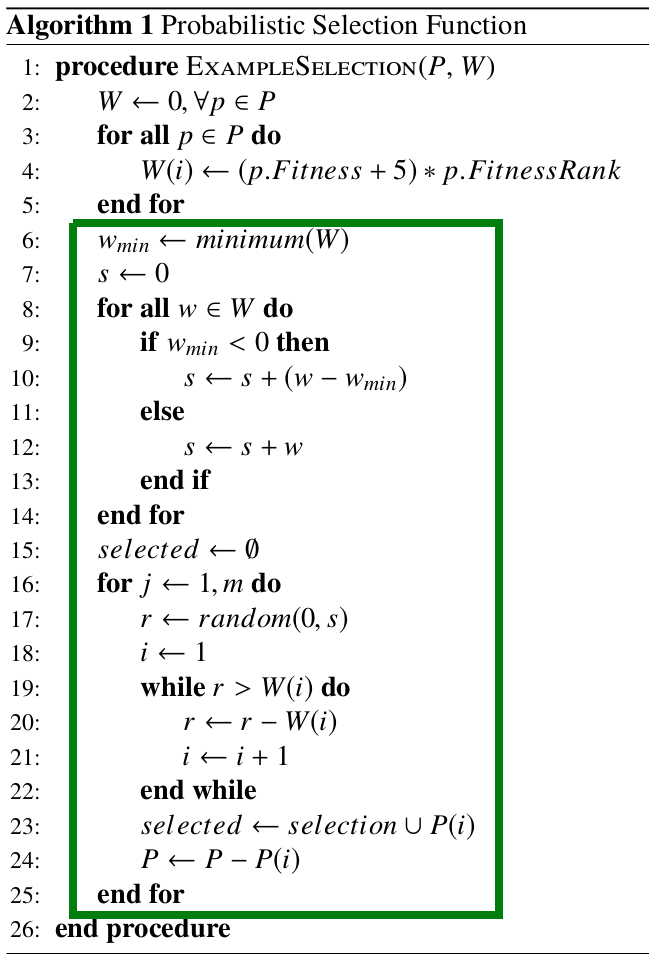
\includegraphics[height=0.8\paperheight]{example_eppsea_code_green_highlight}		
		\end{column}
		\begin{column}{0.5\textwidth}
			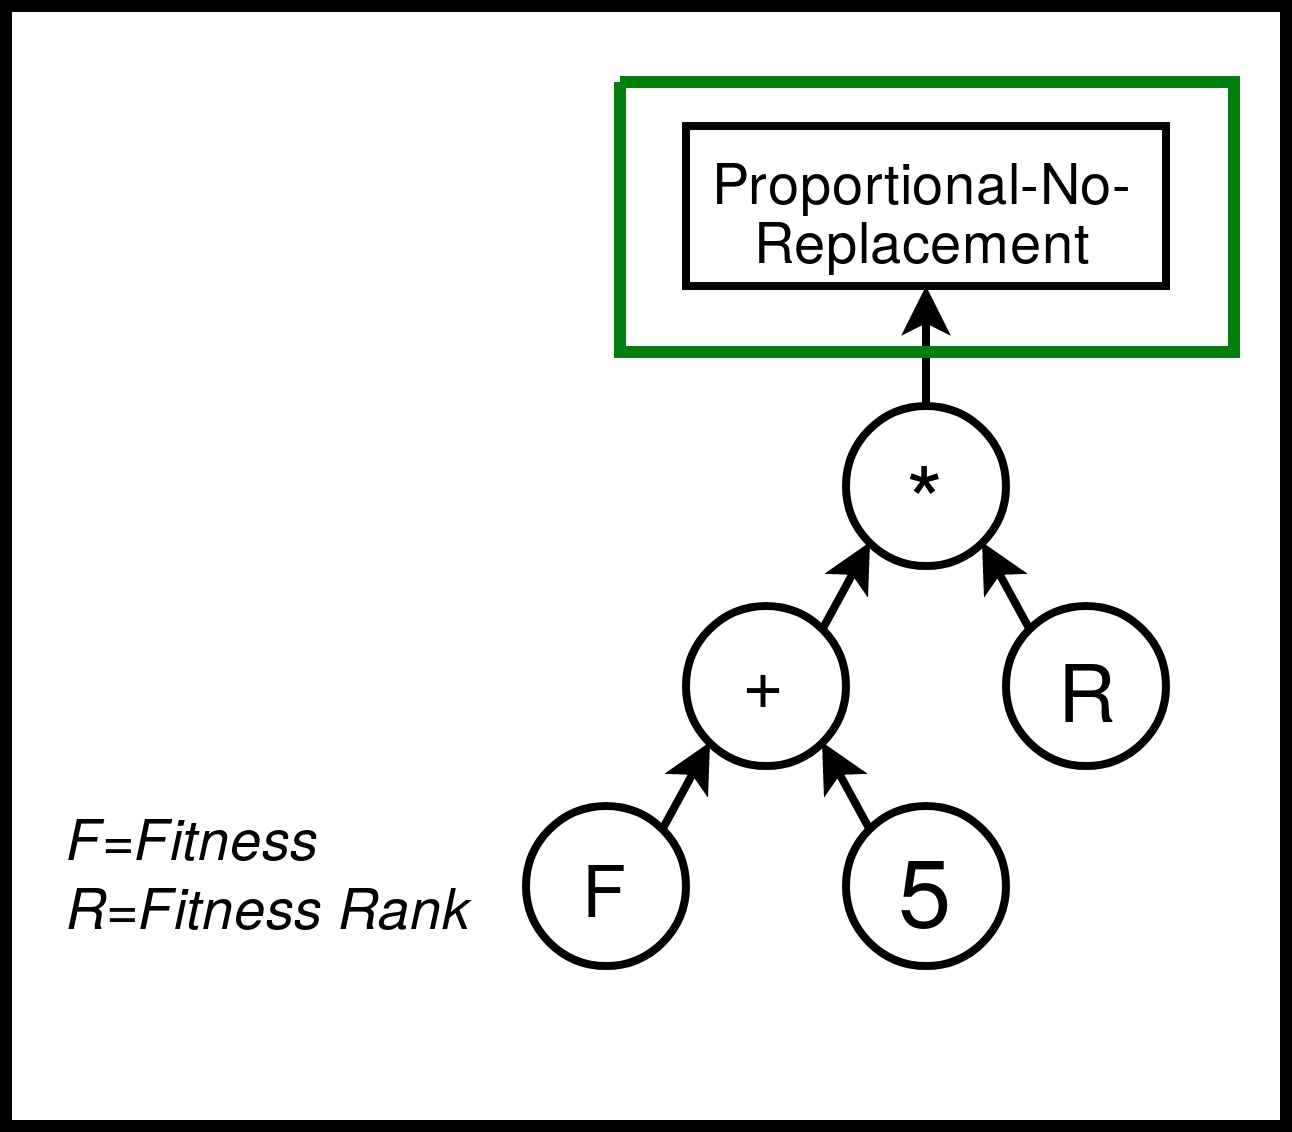
\includegraphics[width=\textwidth]{example_eppsea_no_forks_green_highlight}		
		\end{column}
		\end{columns}		

	\end{frame}			
	
	\begin{frame}
		\begin{itemize}
			 \item<1-|alert@1> The components are evolved together in one genome to form one selection function, and selection functions can be evolved together to tune multiple selection steps of an EA (e.g., parent and survival selection) together
			 \item<2-|alert@2> The GP-Tree is evolved with a generative Hyper-heuristic, exploring a large, yet restricted, space of mathematical functions
			 \item<3-|alert@3> The selection method is evolved with a perturbative Hyper-heuristic, picking from a list of methods inspired by conventional selection functions
		
		\end{itemize}
	\end{frame}	
	
	\begin{frame}
		\frametitle{Representation}
		
		\begin{itemize}
			 \item<1-|alert@1> This format allows us a more manageable search space of selection functions, while also being robust enough to represent both conventional selection functions and a wide variety of new selection functions
			 \item<2-|alert@2> In addition, we can guarantee that all functions in this space are valid selection functions
			 \item<3-|alert@3> This format cannot represent all possible selections, but this is an acceptable trade-off for the more easily-searchable space of selection functions
		\end{itemize}
	\end{frame}		
	
%--------------------------TERMINALS

	\begin{frame}
		\frametitle{Representation - Terminals}
		
		\begin{table}
		\centering
		  \label{tab:gp-terminals1}
		  \begin{tabular}{p{3.5cm}|p{6.5cm}}
		  \hline
		    \textbf{Terminal} & \textbf{Description}\\
		    \hline
		    Fitness &  Individual's fitness value \\
		    \hline
		    Fitness Rank &  Rank assigned to the individual when the population is sorted by fitness (higher fitness = higher rank) \\    
		    \hline
		    Relative Fitness &  Individual's fitness value, minus the minimum fitness value in the population, divided by the range of the population fitness values \\
		    \hline
		    Birth Generation &  Generation number that the individual first appeared in the population \\  
		    \hline             
		    
		\end{tabular}
		\end{table}		
	\end{frame}
	
	\begin{frame}
		\frametitle{Representation - Terminals}
		
		\begin{table}
		\centering
		  \label{tab:gp-terminals2}
		  \begin{tabular}{p{3.5cm}|p{6.5cm}}
		  \hline
		    \textbf{Terminal} & \textbf{Description}\\
		    \hline
		    Relative Uniqueness &  Cartesian distance between the individual's genome and the centroid of all genomes in the population. \\  
		    \hline		    
		    Population Size &  Number of individuals in the population \\
		    \hline
		    Min Fitness &  Smallest fitness value in the population \\
		    \hline
		    Max Fitness &  Largest fitness value in the population \\ 
		    \hline
		    Sum Fitness &  Sum of all fitness values in the population \\
		    \hline
		    Generation Number &  Number of generations of individuals that have been evaluated since the beginning of evolution \\  
		    \hline            
		    
		\end{tabular}
		\end{table}		
	\end{frame}	
	
	\begin{frame}
		\frametitle{Representation - Terminals}
		
		\begin{table}
		\centering
		  \label{tab:gp-terminals3}
		  \begin{tabular}{p{3cm}|p{7cm}}
		  \hline
		    \textbf{Terminal} & \textbf{Description}\\
		    \hline
			    Constant &  Returns a constant number, which is generated from a uniform selection within a configured range when the selection function is generated and held constant for the entire lifetime of the selection function. \\
			    \hline
			    Random &  Returns a random number, which is generated from a uniform selection within a configured range every time selection is performed. \\     
			    \hline      
		    
		\end{tabular}
		\end{table}		
	\end{frame}			
	
% ---------------------------OPERATORS	
	
	\begin{frame}
		\frametitle{Representation - Operators}
		
		\begin{table}
		\centering
		  \label{tab:gp-operators1}
		  \begin{tabular}{p{1.5cm}|c|p{6cm}}
			  \hline
			    \textbf{Operator} & \textbf{Operands} & \textbf{Description}\\
			    \hline
			    + & 2 & Adds the left and right operands. \\
			    \hline
			    - & 2 & Subtracts the right operand from the left operand.\\    
			    \hline
			    * & 2 & Multiplies the left and right operands.\\  
			    \hline
			    / & 2 & Divides the left operand by the right operand. If the right operand is 0, the left operand is instead divided by a very small number, returning a large number while preserving the sign of the dividend.\\      
			    \hline
			    Min & 2 & Returns the minimum of the left and right operands.\\
			    \hline				       
		    
		\end{tabular}
		\end{table}		
	\end{frame}
	
	\begin{frame}
		\frametitle{Representation - Operators}
		
		\begin{table}
		\centering
		  \label{tab:gp-operators2}
		  \begin{tabular}{p{1.5cm}|c|p{6cm}}
			  \hline
			    \textbf{Operator} & \textbf{Operands} & \textbf{Description}\\
			    \hline
			    Max & 2 & Returns the maximum of the left and right operands.\\
			    \hline   
			    Step & 2 & Returns 1 if the left operand is greater than or equal to the right operand, and 0 otherwise.\\
			    \hline
			    Absolute Value & 1 & Returns the absolute value of the operand.\\    
			    \hline				    
                
		    
		\end{tabular}
		\end{table}		
	\end{frame}		
	
% ---------------------------SELECTION METHODS	
	\begin{frame}
		\frametitle{Representation - Selection Methods}
		
		\begin{table}
		\centering
		  \label{tab:selection-methods1}
		  \begin{tabular}{p{3cm}|p{7cm}}
		  \hline
		    \textbf{Method} & \textbf{Description}\\
			    \hline
			    Proportional-Replacement & A weighted random selection, with each individual's weight equal to its desirability score \\
			    \hline
			    Proportional-No-Replacement & As with Proportional-Replacement, but an individual is removed from the selection pool after being selected\\
			    \hline
			    \textit{k}-Tournament-Replacement& A random subset of \textit{k} individuals is considered, and the individual with the highest desirability score in the subset is selected \\
			    \hline
			    \textit{k}-Tournament-No-Replacement & As with \textit{k}-Tournament-Replacement, but an individual is removed from the selection pool after being selected\\
			    \hline
		\end{tabular}
		\end{table}		
	\end{frame}	
	
	
	\begin{frame}
		\frametitle{Representation - Selection Methods}
		
		\begin{table}
		\centering
		  \label{tab:selection-methods2}
		  \begin{tabular}{p{3cm}|p{7cm}}
		    \textbf{Method} & \textbf{Description}\\
			    \hline
				Truncation & Individuals with the highest desirability score are selected, with no individual being selected more than once \\
				\hline
				Stochastic-Universal-Sampling & A variant of proportional selection that chooses individuals at evenly spaced intervals, reducing sampling bias\\	
				\hline	    
		\end{tabular}
		\end{table}		
	\end{frame}		
% ---------------------------EXAMPLES	
	
	\begin{frame}
		\frametitle{Representation - Example}
		Selection Function: $(Fitness + 5) * FitnessRank \rightarrow$ Proportional-No-Replacement
		\begin{table}
			\begin{tabular}{ m{5cm} | c | c | c | c }
				Population Member & 1 & 2 & 3 & 4  \\
				\hline
				Fitness & 300 & 250 & 200 & 350  \\
				Fitness Rank & 3 & 2 & 1 & 4 \\
				& & & & \\ 
				& & & & \\
			\end{tabular}
		\end{table}		
	\end{frame}	
	
	\begin{frame}
		\frametitle{Representation - Example}
		Selection Function: $(Fitness + 5) * FitnessRank \rightarrow$ Proportional-No-Replacement
		\begin{table}
			\begin{tabular}{ m{5cm} | c | c | c | c }
				Population Member & 1 & 2 & 3 & 4  \\
				\hline
				Fitness & 300 & 250 & 200 & 350  \\
				Fitness Rank & 3 & 2 & 1 & 4 \\
				\hline
				$Fitness + 5$ & 305 & 255 & 205 & 355 \\ 
				& & & & \\ 
			\end{tabular}
		\end{table}		
	\end{frame} 
	
	\begin{frame}
		\frametitle{Representation - Example}
		Selection Function: $(Fitness + 5) * FitnessRank \rightarrow$ Proportional-No-Replacement
		\begin{table}
			\begin{tabular}{ m{5cm} | c | c | c | c }
				Population Member & 1 & 2 & 3 & 4  \\
				\hline
				Fitness & 300 & 250 & 200 & 350  \\
				Fitness Rank & 3 & 2 & 1 & 4 \\
				\hline
				$Fitness + 5$ & 305 & 255 & 205 & 355 \\ 
				$(Fitness + 5) * FitnessRank$ & 915 & 510 & 205 & 1420 \\
			\end{tabular}
		\end{table}		
	\end{frame} 
	
	\begin{frame}
		\frametitle{Representation - Example}
		Selection Function: $(Fitness + 5) * FitnessRank \rightarrow$ Proportional-No-Replacement
		\begin{table}
			\begin{tabular}{ m{5cm} | c | c | c | c }
				Population Member & 1 & 2 & 3 & 4  \\
				\hline
				Fitness & 300 & 250 & 200 & 350  \\
				Fitness Rank & 3 & 2 & 1 & 4 \\
				\hline
				$Fitness + 5$ & 305 & 255 & 205 & 355 \\ 
				$(Fitness + 5) * FitnessRank$ & 915 & 510 & 205 & 1420 \\
			\end{tabular}
		\end{table}	
		Desirability scores: 915, 510, 205, 1420. Individuals are selected with probability proportional to their desirability score.	
	\end{frame} 			 
	
	\begin{frame}
		\frametitle{Representation - Example}
		Selection Function: $ FitnessRanking*100 / (100-Fitness) \rightarrow$ \textit{k}-tournament, \textit{k}=3
		\begin{table}
			\begin{tabular}{ m{5cm} | c | c | c | c }
				Population Member & 1 & 2 & 3 & 4  \\
				\hline
				Fitness & 300 & 250 & 200 & 350  \\
				Fitness Rank & 3 & 2 & 1 & 4 \\
				$ FitnessRanking*100 / (100-Fitness)$ & -1.5 & -1.33 & -1.0 & -1.6 \\ 
			\end{tabular}
		\end{table}
		Desirability scores: -1.5, -1.33, -1.0, -1.6. Selection picks a random set of three individuals, and selects the individual among them with the highest desirability.
	\end{frame}	
	
	\begin{frame}
		\frametitle{Meta-EA}
		
		\begin{itemize}
			 \item<1-|alert@1> We use Koza-style GP to evolve the trees representing the selection functions
			 \item<2-|alert@2> Each function is evaluated by running an EA utilizing that function on a fixed set of benchmark instances from a selected problem class	
			 \item<3-|alert@3> The best fitness reached by the EA, averaged over all runs and across all problem instances, is assigned as the fitness of the selection function at the meta-EA level 		 
			 \item<4-|alert@4> After the meta-EA is run, the selection strategies are tested for generalization on a separate set of ``testing'' instances from the same problem class
		\end{itemize}
	\end{frame}
	
%---------------------------INITIAL EXPERIMENT

	\begin{frame}
		\frametitle{Initial Experiment}
		
		\begin{itemize}
			 \item<1-|alert@1> Our initial experiment used an early version of the methodology to test our approach
			 \item<2-|alert@2> We built a basic EA, with simple parent selection, recombination, survival selection, and mutation
			 \item<3-|alert@3> We targeted improvement of the parent selection stage of the meta-EA, keeping all other factors constant			 
			 \item<4-|alert@4> Survival selection is performed randomly, so that the parent selection would have to provide 100\% of the selection pressure
			 \item<5-|alert@5> For our benchmark problem class, we used the NK-Landscape problem class		 
		\end{itemize}
	\end{frame}

	\begin{frame}
		\frametitle{Initial Experiment - Results}
		\begin{columns}
		\begin{column}{0.4\textwidth}
			Our meta-EA evolved a parent selection function that significantly outperformed typical selection on 46 of the 50 benchmark functions we tested.
		\end{column}
		\begin{column}{0.6\textwidth}
			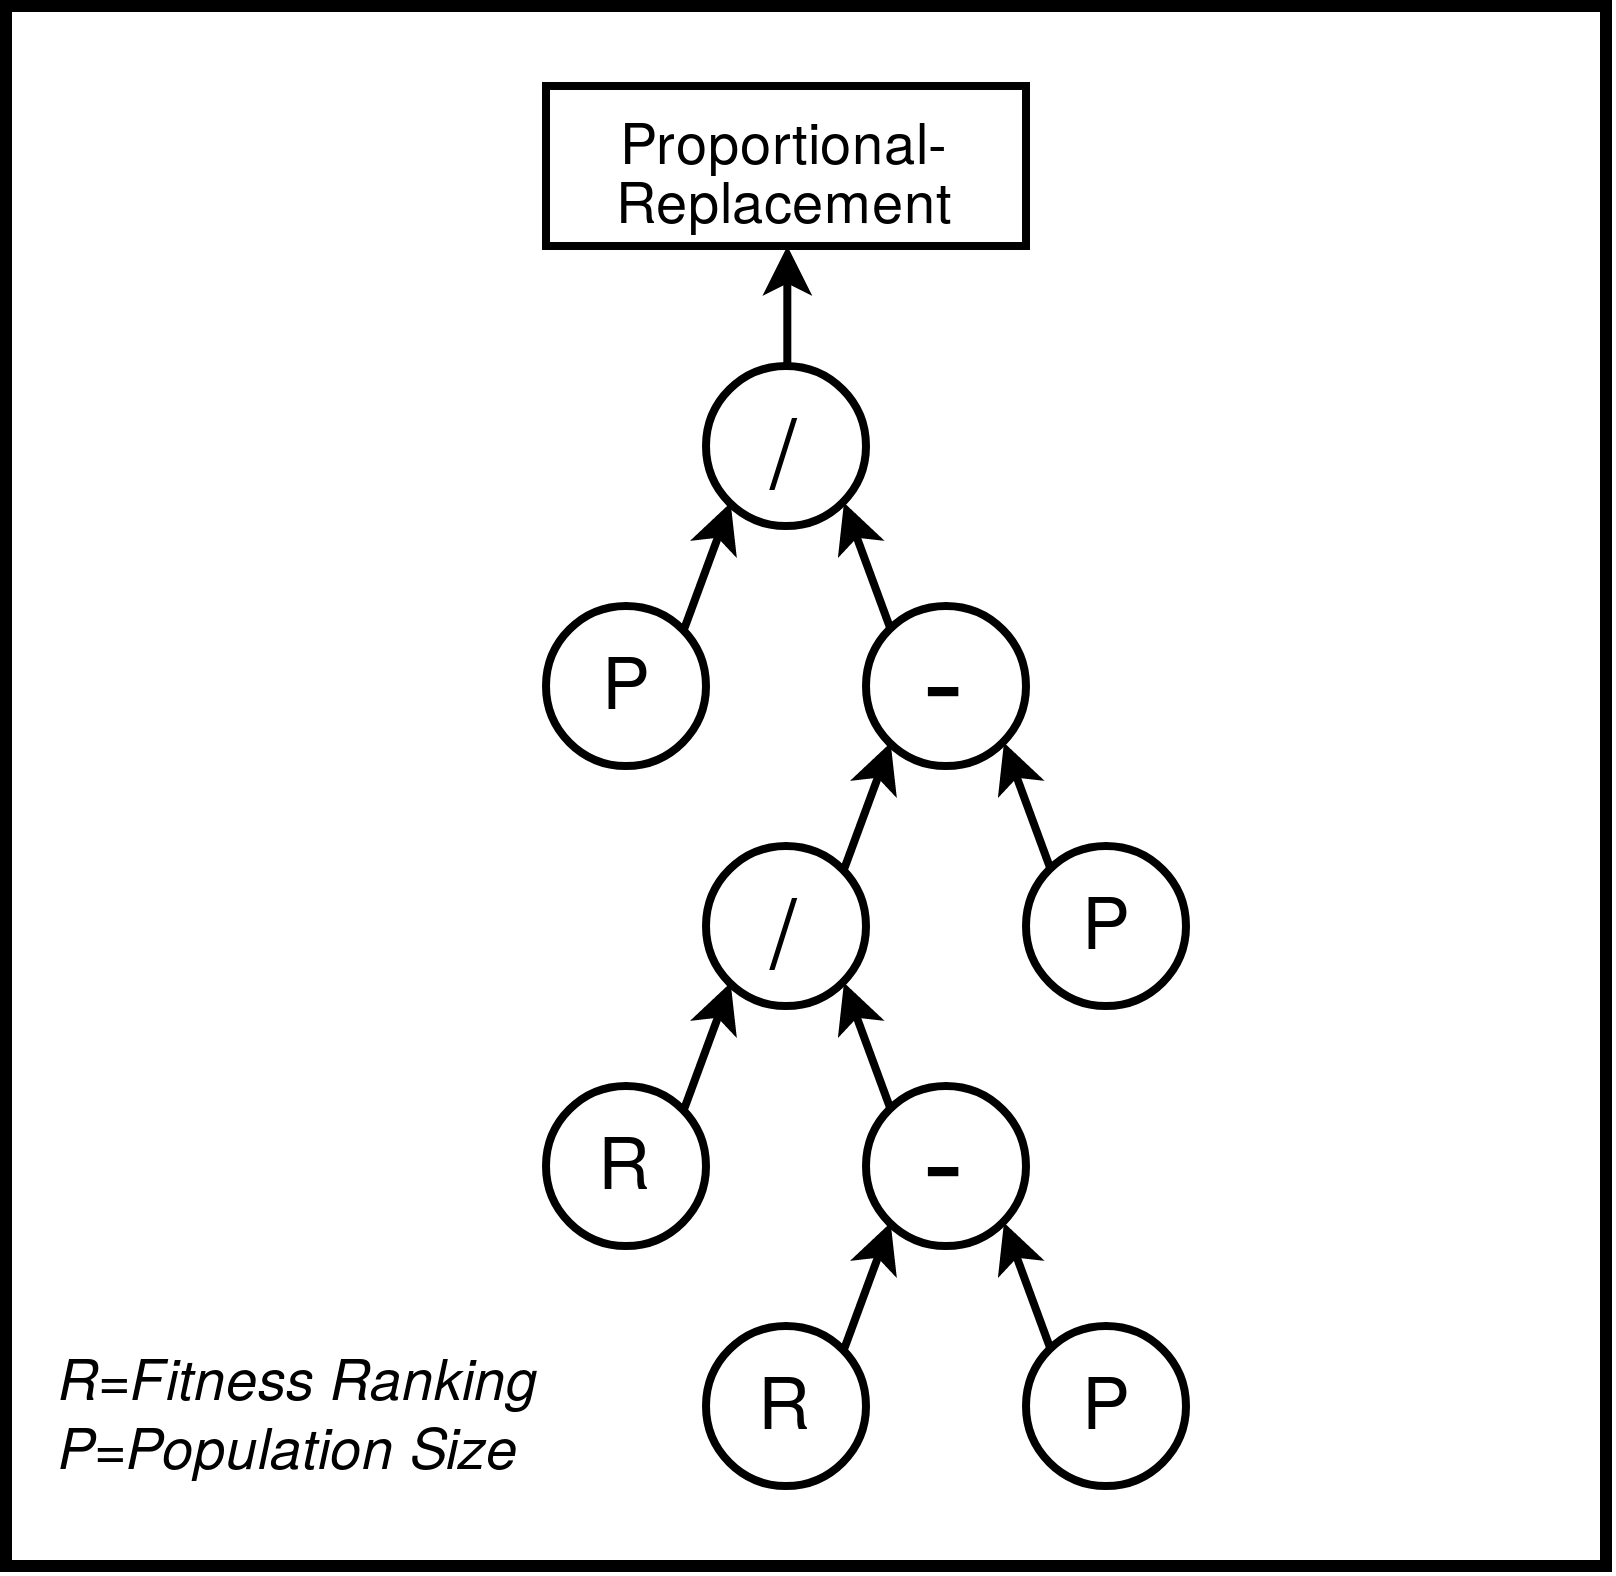
\includegraphics[width=\textwidth]{initialExperimentResult}
		\end{column}
		\end{columns}
	\end{frame}

	\begin{frame}
		\centering
		\frametitle{Initial Experiment - Results}
		Best fitness vs. EA evals, averaged over all runs:
		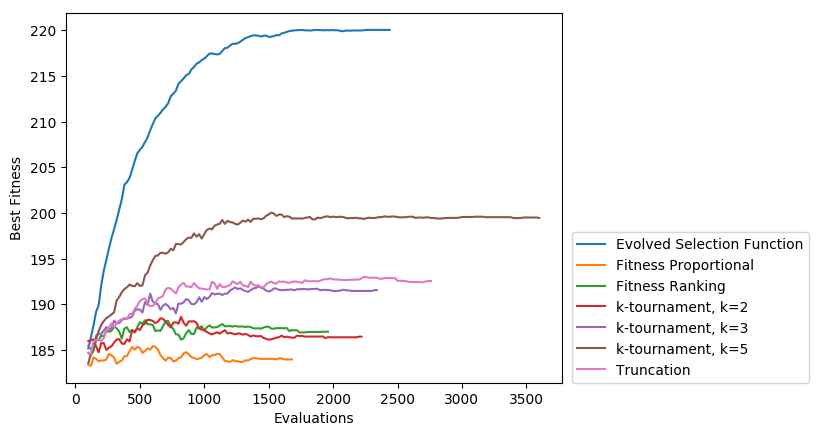
\includegraphics[width=\textwidth]{nk_landscape_fitness_plot}
	\end{frame}	
	
	\begin{frame}
		\centering
		\frametitle{Initial Experiment - Results}
		Final best fitnesses achieved by the EA:		
		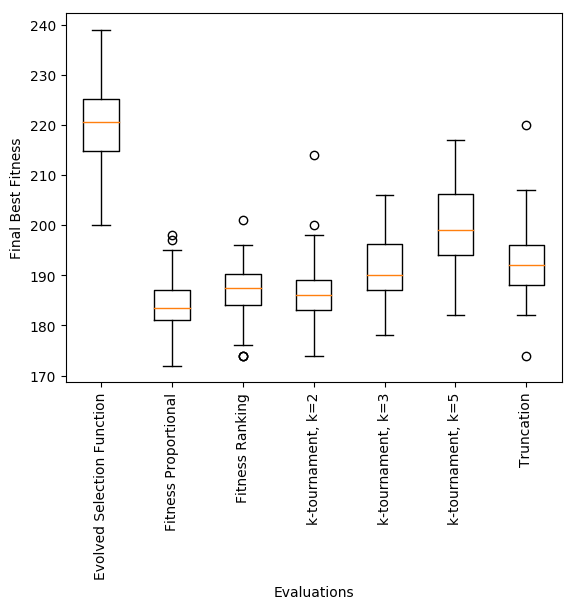
\includegraphics[height=0.8\textheight]{nk_landscape_boxplot}
	\end{frame}	
	
	\begin{frame}
		\frametitle{Initial Experiment - Takeaways}
		Takeaways from our initial experiment:
		\begin{itemize}
			 \item<2-|alert@2> Our Hyper-heuristic works! We successfully evolved a new selection function for the EA, specialized to the NK problem class, that outperforms conventional selection methods. We published this work in the ECADA Workshop at GECCO 2018
			 \item<3-|alert@3> We next needed to test the method against a parameter-tuned EA		 
			 \item<4-|alert@4> We also needed to show that our methodology works with other problem classes, and other EAs
			 \item<5-|alert@5> We built these takeaways into our next three experiments
		\end{itemize}
	\end{frame}	
	
% ------------------------MAIN EXPERIMENTS
 
	\begin{frame}
		\frametitle{Main Experiments}
		We tested the most recent version of our methodology with three experiments
		\begin{itemize}
			 \item<2-|alert@2> Evolving both parent and survival selection for a basic EA, solving MK-Landscapes
			 \item<3-|alert@3> Evolving both parent and survival selection for a basic EA, solving real-valued benchmark functions
			 \item<4-|alert@4> Evolving a new mean-update scheme for CMA-ES, solving real-valued benchmark functions
		\end{itemize}
	\end{frame}	 
 
% --------------------------------------------------EXPERIMENT 1 
 
	\begin{frame}
		\frametitle{Experiment 1}
		
		\begin{itemize}
			 \item<1-|alert@1> We use the same basic EA as in our initial experiment, but we evolve parent and survival selection together in one genome
			 \item<2-|alert@2> We use the iRace tuning package to find the best set of parameters to run the EA with, including the best choice of parent and survival selection from a list of conventional selection functions
			 \item<3-|alert@3> We use the MK-Landscape problem class, a generalization of the NK-Landscape class			 
			 \item<4-|alert@4> At the end of the meta-EA, we test the evolved selection function against the conventional selection functions selected by iRace
		\end{itemize}
	\end{frame} 
	
	\begin{frame}
		\frametitle{Experiment 1 - Results}
		Results: Our meta-EA evolved a parent selection function that significantly outperformed typical selection on 45 of the 50 benchmark functions we tested.
	\end{frame} 
	
	\begin{frame}
		\frametitle{Experiment 1 - Results}
		Best fitness vs. EA evals, averaged over all runs:		
		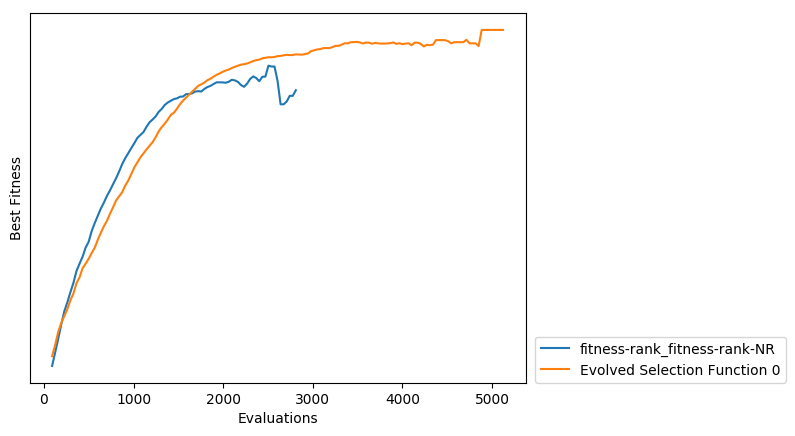
\includegraphics[width=\textwidth]{Experiment1LinePlot}
	\end{frame} 	
	
	\begin{frame}
		\frametitle{Experiment 1 - Results}
		\centering
		Final best fitnesses achieved by the EA:
		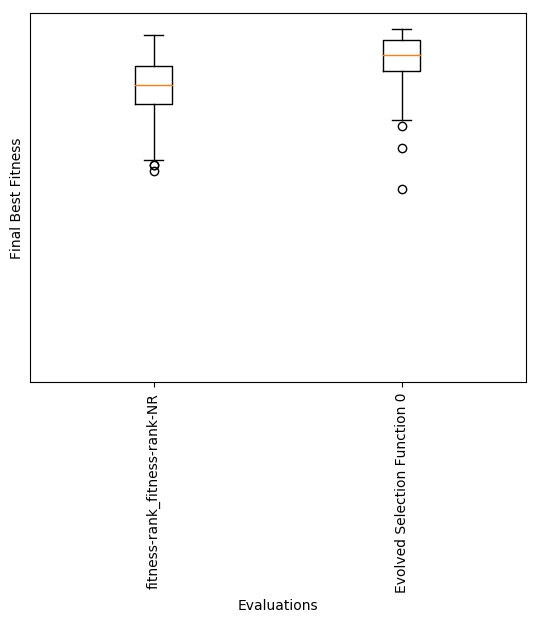
\includegraphics[height=0.8\textheight]{Experiment1Boxplot}
	\end{frame} 	
	
	\begin{frame}
		\frametitle{Experiment 1 - Results}
		Parent Selection of the best evolved selection function:
		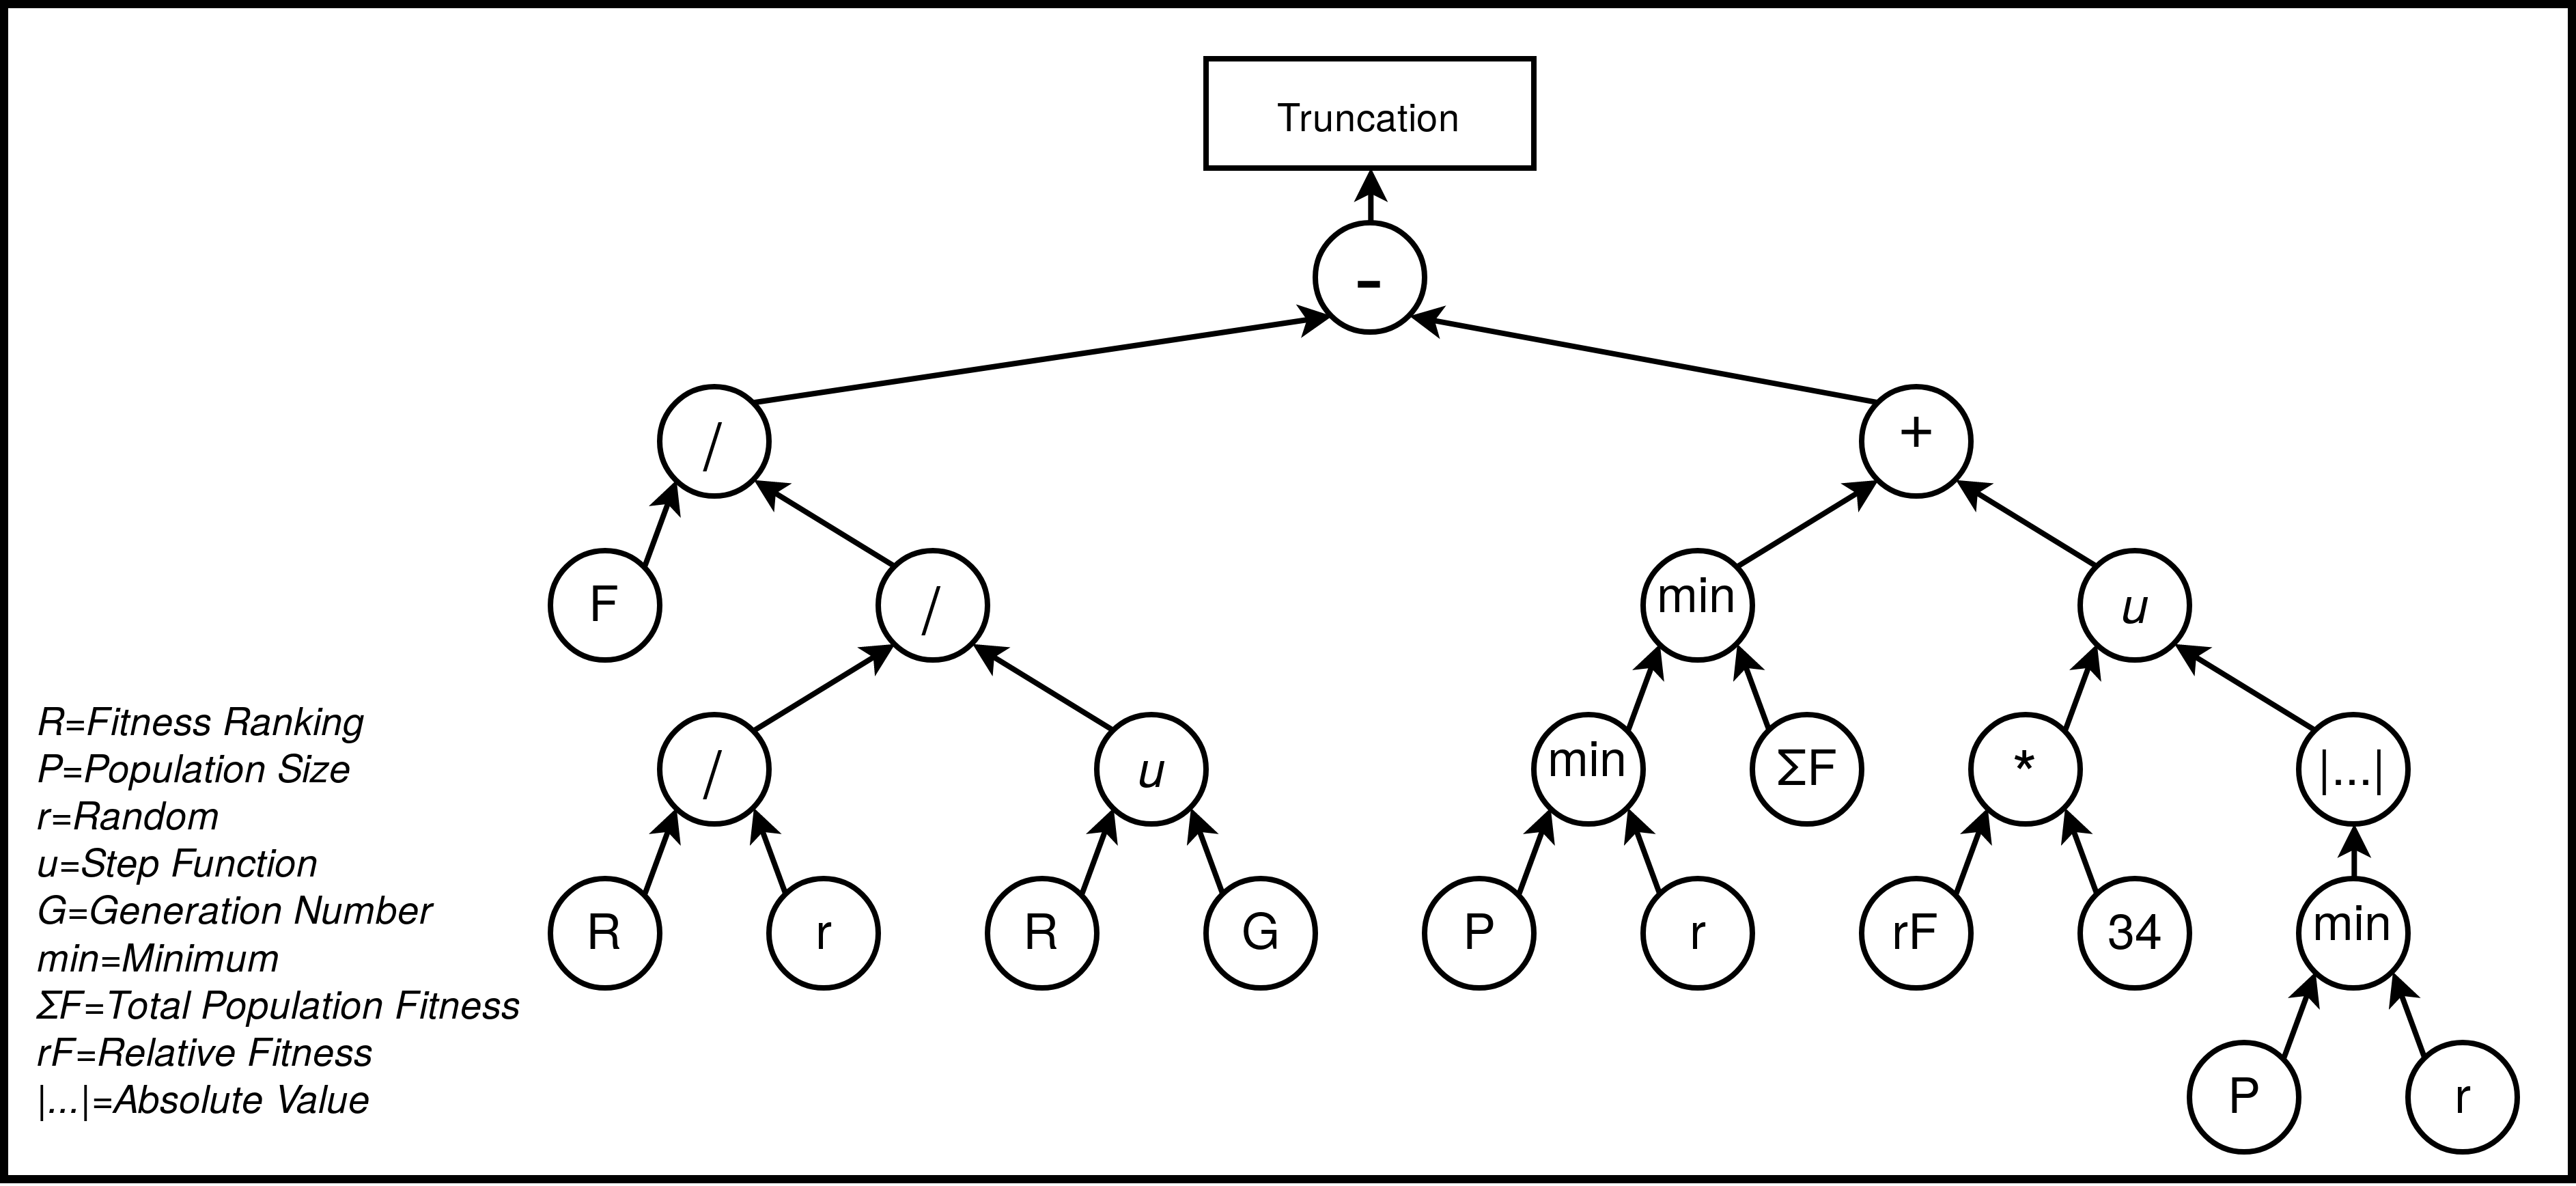
\includegraphics[width=\textwidth]{experiment1Result}
	\end{frame} 
	
	\begin{frame}
		\frametitle{Experiment 1 - Takeaways}
		Experiment 1 Takeaways
		\begin{itemize}
			 \item<1-|alert@1> Our Hyper-heuristic performs well, even against state-of-the-art parameter tuning
			 \item<2-|alert@2> Next, we need to test against more benchmark functions
		\end{itemize}
	\end{frame} 		
 
% ----------------------------------------EXPERIMENT 2

	\begin{frame}
		\frametitle{Experiment 2}
		
		\begin{itemize}
			 \item<1-|alert@1> We use the same basic EA as in Experiment 1, still evolving parent and survival selection together
			 \item<2-|alert@2> For benchmark functions, we use the 24 real-valued functions in the Comparing Continuous Optimizers package, running the meta-EA on each function separately. We use all available the available 10-dimensional instances for each function, setting aside some for testing generalization
			 \item<3-|alert@3> We still use iRace to find the optimal parameter set for each function.
			 \item<4-|alert@4> As with Experiment 1, we test for generalization at the end of the meta-EA
		\end{itemize}
	\end{frame} 
	
	\begin{frame}
		\frametitle{Experiment 2}
		\centering
		COCO F \#15: Rastrigin Function
		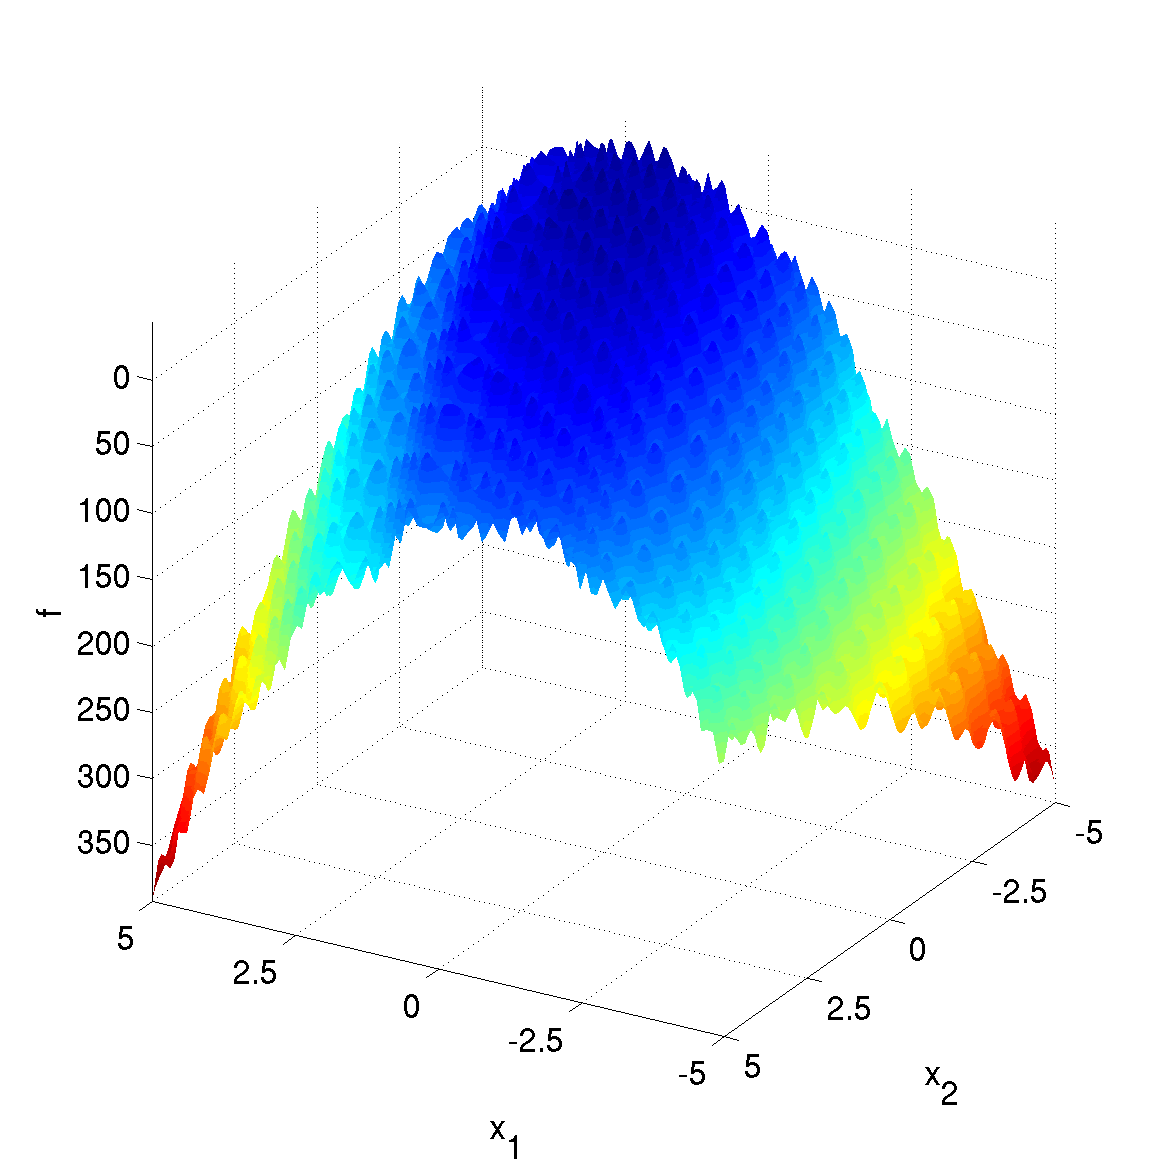
\includegraphics[height=0.8\textheight]{rastrigin_landscape}
	\end{frame}	
	
	\begin{frame}
		\centering	
		\frametitle{Experiment 2}
		COCO F \#21: Gallagher's Gaussian 101-me Peaks Function
		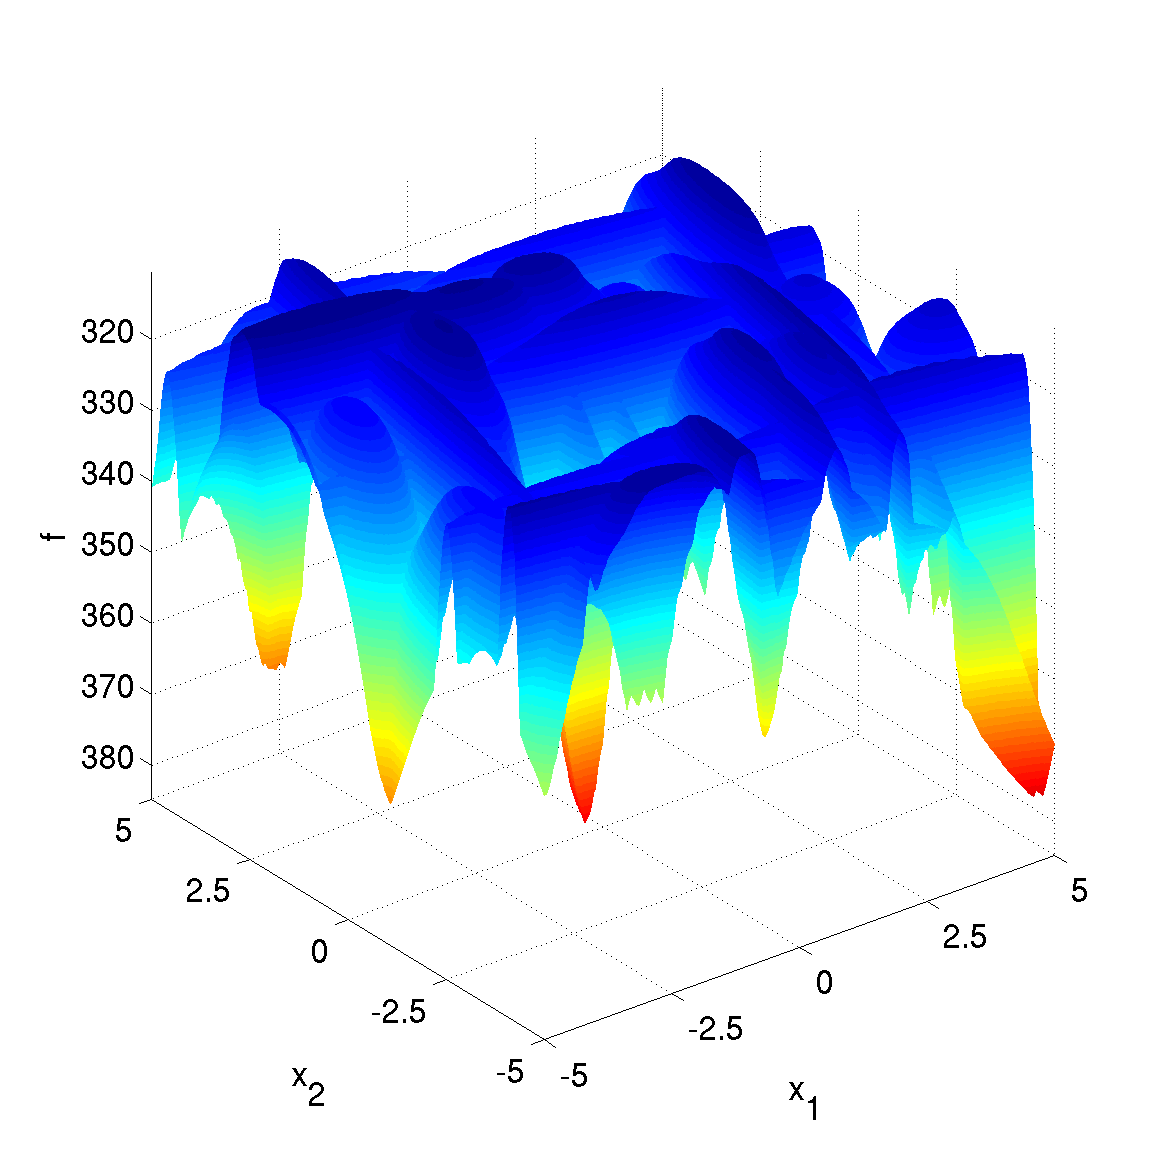
\includegraphics[height=0.8\textheight]{gallagher_landscape}
	\end{frame}		
	
	\begin{frame}
		\centering	
		\frametitle{Experiment 2}
		COCO F \#23: Katsuura Function
		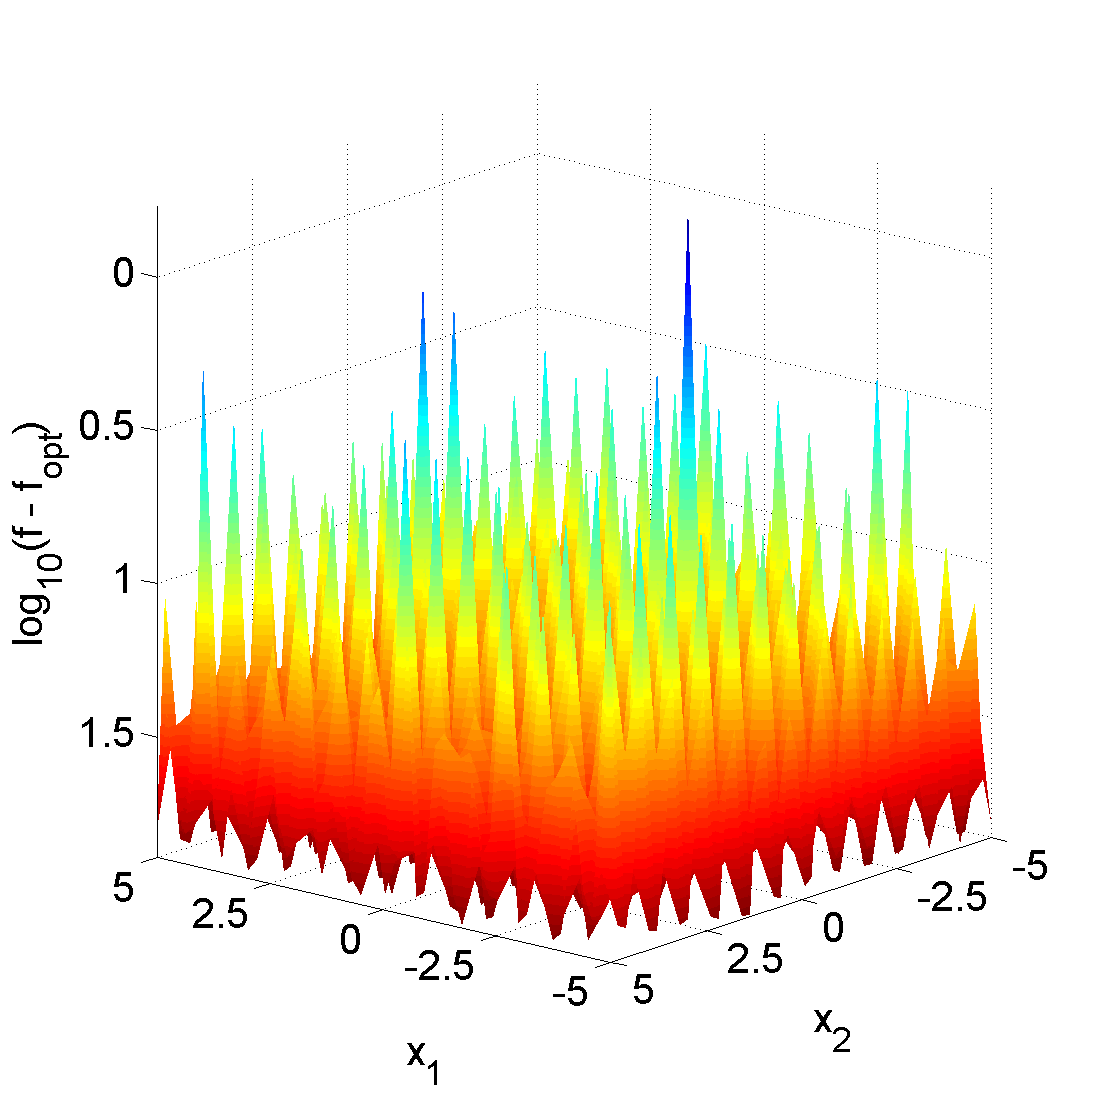
\includegraphics[height=0.8\textheight]{katsuura_landscape}
	\end{frame}		
	
	\begin{frame}
	Results:
		\frametitle{Experiment 2 - Results}
		\begin{itemize}
			 \item<2-|alert@2> For 17 of the 24 function classes, the evolved selection function significantly outperformed the conventional selection on at least 1 problem instance
			 \item<3-|alert@3> For 6 of the 24 function classes, the evolved selection function significantly outperformed the conventional selection on at least half of the problem instances
			 \item<4-|alert@4> For 2 of the 24 function classes, the evolved selection function significantly outperformed the conventional selection on all of the problem instances
		\end{itemize}
		
	\end{frame} 
	
	\begin{frame}
	Results:
	\begin{table}
	\centering
	  \label{tab:experiment2results}
	  \begin{tabular}{cc}
		Problem Index (D=10) & Number of Instances Improved \\
		\hline
		F=1 & 0 / 12 \\
		\hline
		F=2 & 1 / 12 \\
		\hline
		F=3 & 2 / 12 \\
		\hline
		F=4 & 2 / 12 \\
		\hline
		F=5 & 5 / 12 \\
		\hline
		F=6 & 2 / 12 \\
		\hline
		F=7 & 7 / 12 \\
		\hline
		F=8 & 2 / 12 \\
		\hline
		F=9 & 12 / 12 \\
		\hline
		F=10 & 1 / 12 \\
		\hline
		F=11 & 7 / 12 \\
		\hline
		F=12 & 0 / 12 \\                     	
	  \hline
	\end{tabular}
	\end{table}		
	
	\end{frame} 
	
	\begin{frame}
	Results:
	\begin{table}
	\centering
	  \label{tab:experiment2results}
	  \begin{tabular}{cc}
		Problem Index (D=10) & Number of Instances Improved \\
		\hline
		F=13 & 2 / 12 \\
		\hline
		F=14 & 0 / 12 \\
		\hline
		F=15 & 0 / 12 \\
		\hline
		F=16 & 0 / 12 \\
		\hline
		F=17 & 4 / 12 \\
		\hline
		F=18 & 4 / 12 \\
		\hline
		F=19 & 12 / 12 \\
		\hline
		F=20 & 0 / 12 \\
		\hline
		F=21 & 8 / 12 \\
		\hline
		F=22 & 6 / 12 \\
		\hline
		F=23 & 0 / 12 \\
		\hline
		F=24 & 1 / 12 \\                       
		
	  \hline
	\end{tabular}
	\end{table}		
	
	\end{frame}	
	
	\begin{frame}
		\frametitle{Experiment 2 - Takeaways}
		Experiment 2 Takeaways
		\begin{itemize}
			 \item<1-|alert@1> Unfortunately, Our Hyper-heuristic did not perform well for many of the benchmarks tested. In some cases, the evolved selection function performed worse
			 \item<2-|alert@2> This could be due to overspecialization to ``training instances''
			 \item<3-|alert@3> Our suspicion: some functions ``too easy''; only need some kind of selection pressure 
			 \begin{itemize}
			 	\item<4-|alert@4> We saw little improvement on the original Rosenbrock function (F=8), but universal improvement on the rotated Rosenbrock Function.
			 \end{itemize}
			 \item<5-|alert@5> Other functions ``too hard''; need an entirely new evolution strategy to see significant gains
			 \begin{itemize}
			 	\item<6-|alert@6> Little improvement on functions with weak global structure, which our EA setup depends on
			 \end{itemize}			 
			 \item<7-|alert@7> Using the same dimensionality for all 24 problems would inherently lead to ``easy'' and ``hard'' problems			 
		\end{itemize}
	\end{frame} 	
 
% -----------------------------EXPERIMENT 3

	\begin{frame}
		\frametitle{Experiment 3}
		
		\begin{itemize}
			 \item<1-|alert@1> For our third experiment, we chose a new EA: Covariance Matrix Adaptation Evolutionary Strategy (CMA-ES)
			 \begin{itemize}
			 	\item<2-|alert@2> Mostly parameterless ES that moves a sampling mean through the fitness space, samples points around it, and updates mean
			 	\item<3-|alert@3> Much more State-of-the-Art, w/ better performance than our basic EA
			 	\item<4-|alert@4> Able to find the global optimum of some of the COCO function classes
			 \end{itemize}
			 \item<5-|alert@5> We targeted the mean-update function of CMA-ES, to better select the points used for updating the mean (normally truncation)
			 \item<6-|alert@6> We select the COCO functions (class and dimensionality) which CMA-ES is unable to solve more than 50\% of the time
		\end{itemize}
	\end{frame}  
 
	\begin{frame}
	Results:
		\frametitle{Experiment 3 - Results}
		For 6 of the 11 functions tested, the CMA-ES using the evolved selection function found the global best fitness more often than CMA-ES without it
		
	\end{frame} 
		
	\begin{frame}
		\frametitle{Experiment 3 - Results}
		\centering
		F=4,D=2:
		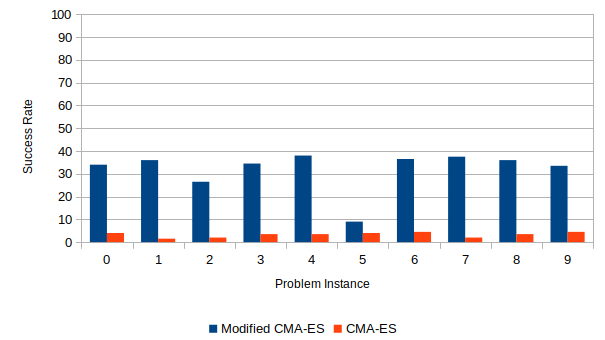
\includegraphics[width=\textwidth]{experiment3_f4d2_bargraph}
	\end{frame} 		
	
	\begin{frame}
		\frametitle{Experiment 3 - Results}
		\centering
		F=19,D=2:
		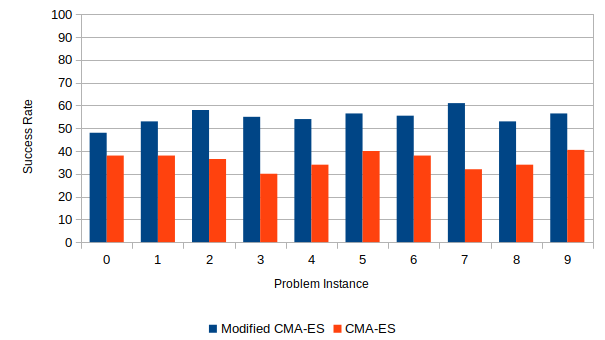
\includegraphics[width=\textwidth]{experiment3_f19d2_bargraph}
	\end{frame} 	
	
	\begin{frame}
		\frametitle{Experiment 3 - Results}
		\centering
		F=20,D=2:
		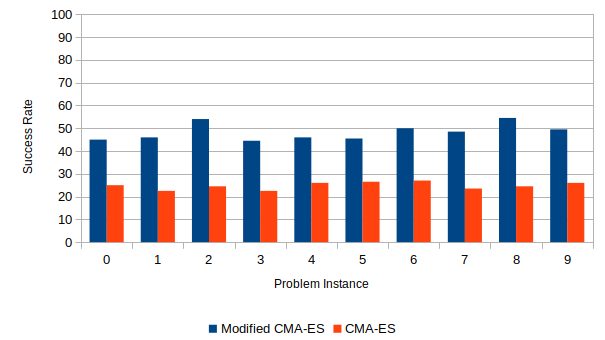
\includegraphics[width=\textwidth]{experiment3_f20d2_bargraph}
	\end{frame} 
	
	\begin{frame}
		\frametitle{Experiment 3 - Results}
		\centering
		F=21,D=2:
		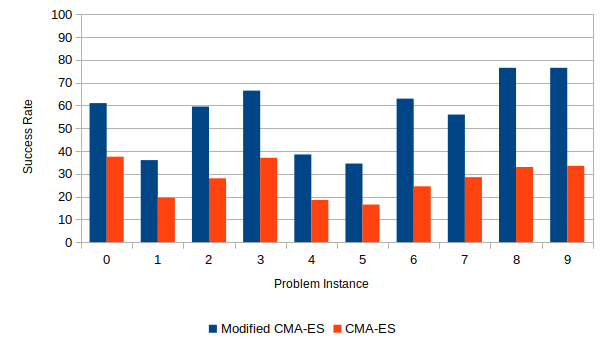
\includegraphics[width=\textwidth]{experiment3_f21d2_bargraph}
	\end{frame} 			
	
	\begin{frame}
		\frametitle{Experiment 3 - Results}
		\centering
		F=12,D=10:
		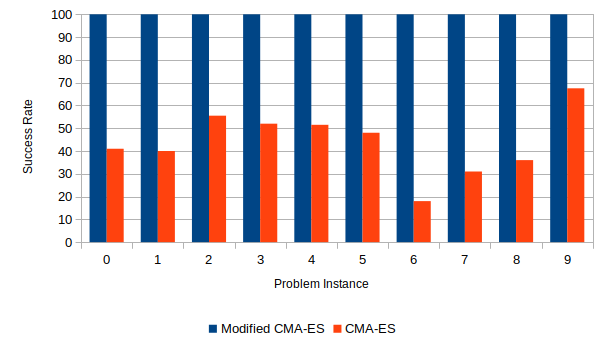
\includegraphics[width=\textwidth]{experiment3_f12d10_bargraph}
	\end{frame} 
	
	\begin{frame}
		\frametitle{Experiment 3 - Results}
		\centering
		F=6,D=10:
		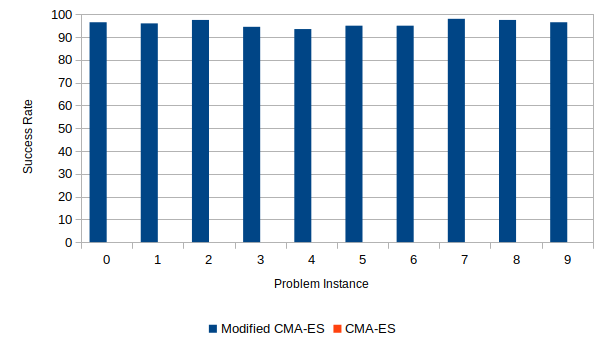
\includegraphics[width=\textwidth]{experiment3_f6d10_bargraph}
	\end{frame} 
	
	
	\begin{frame}
		\frametitle{Experiment 3 - Results}
		\centering
		F=3,D=2:
		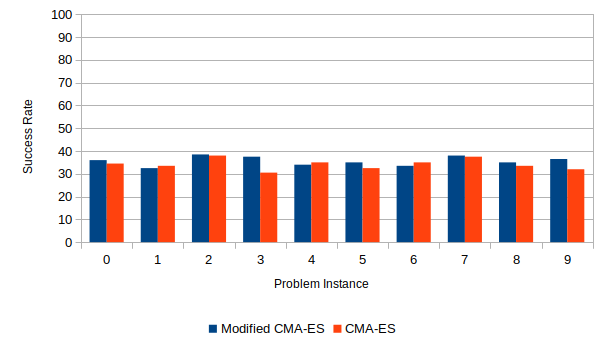
\includegraphics[width=\textwidth]{experiment3_f3d2_bargraph}
	\end{frame}	
		
	
	\begin{frame}
		\frametitle{Experiment 3 - Results}
		\centering
		F=15,D=2:
		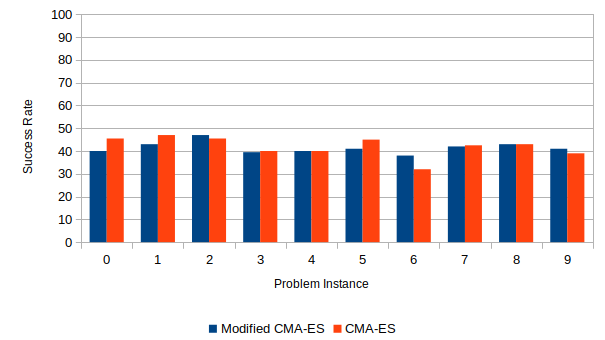
\includegraphics[width=\textwidth]{experiment3_f15d2_bargraph}
	\end{frame}					
 
	\begin{frame}
		\frametitle{Experiment 3 - Results}
		\centering
		F=16,D=10:
		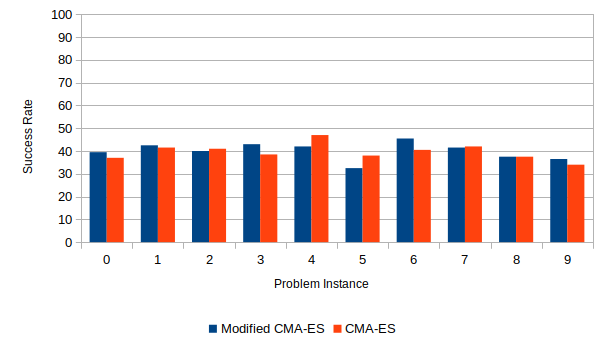
\includegraphics[width=\textwidth]{experiment3_f16d10_bargraph}
	\end{frame}	 
	
	\begin{frame}
		\frametitle{Experiment 3 - Results}
		\centering
		F=23,D=5:
		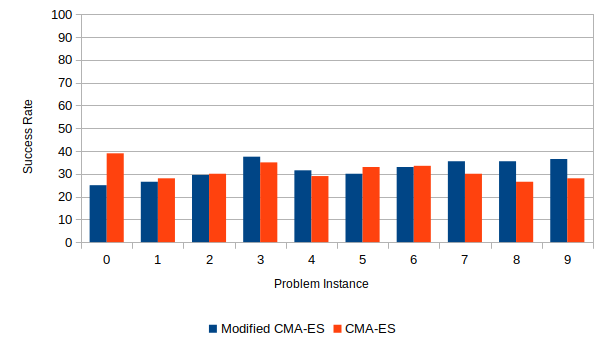
\includegraphics[width=\textwidth]{experiment3_f23d5_bargraph}
	\end{frame}	 
	
	\begin{frame}
		\frametitle{Experiment 3 - Results}
		\centering
		F=24,D=2:
		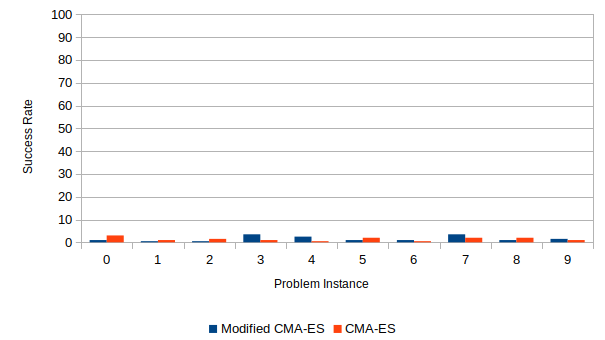
\includegraphics[width=\textwidth]{experiment3_f24d2_bargraph}
	\end{frame}	 
	
	\begin{frame}
		\frametitle{Experiment 3 - Takeaways}
		Experiment 3 Takeaways
		\begin{itemize}
			 \item<1-|alert@1> CMA-ES sees significant--sometimes dramatic--improvement with a new evolved mean update selection function, for some benchmark functions
			 \item<2-|alert@2> Performance on other benchmarks may depend more heavily on other CMA-ES update functions
			 \item<3-|alert@3> Functions with poor performance have poor local structure, require a more intelligence search of global scale (i.e., Rastrigin)		 			 
		\end{itemize}
	\end{frame} 
	
	\begin{frame}
		\frametitle{Final Conclusions}
		Final Conclusions
		\begin{itemize}
			 \item<1-|alert@1> In some cases, there is significant benefit to evolving a new selection function for a particular EA running on a particular benchmark
			 \item<2-|alert@2> Potential performance gain likely depends strongly on the EA, the component being replaced, and the problem being solved		 
		\end{itemize}
	\end{frame} 		
	
	\begin{frame}
		\frametitle{Threats to Validity}
		Threats to Validity
		\begin{itemize}
			 \item<1-|alert@1> We still have yet to test this method on EAs solving real-world problems
			 \item<2-|alert@2> Improvements shown in experiments 1 and 2 were on very basic EA, likely too simple/out of date for real world use	 
			 \item<3-|alert@3> Implementation of CMA-ES in experiment 3 lacked restarts, and some features built into more recent CMA-ES models.	 	
			 \item<4-|alert@4> Some information encodable in GP-Trees is not typically considered for selection, not present in the conventional selection functions tested against.	 					  
		\end{itemize}
	\end{frame} 
	
	\begin{frame}
		\frametitle{Future Work}
		Future Work
		\begin{itemize}
			 \item<1-|alert@1> Investigate methods that do not require as much \textit{a priori} calculation
			 \item<2-|alert@2> Test methodology on EAs solving real-world problems	 
			 \item<3-|alert@3> Test against previous research on evolved selection functions (Grammatical Evolution)	 	
			 \item<4-|alert@4> Test on CMA-ES with more robust features/modern improvements
			 \item<5-|alert@5> Test with more terminals available to GP-Tree in meta-EA, including mate preference information
		\end{itemize}
	\end{frame} 				
 
\end{document}

